\documentclass[tikz]{standalone}
\usepackage{amsmath,amssymb,multirow}
\usetikzlibrary{shapes.misc, positioning,automata,arrows,calc,fit}
\tikzset{VertexStyle/.style = {draw,circle,thick,
		minimum size=1cm,
		font=\Large\bfseries},thick} 
\begin{document}
	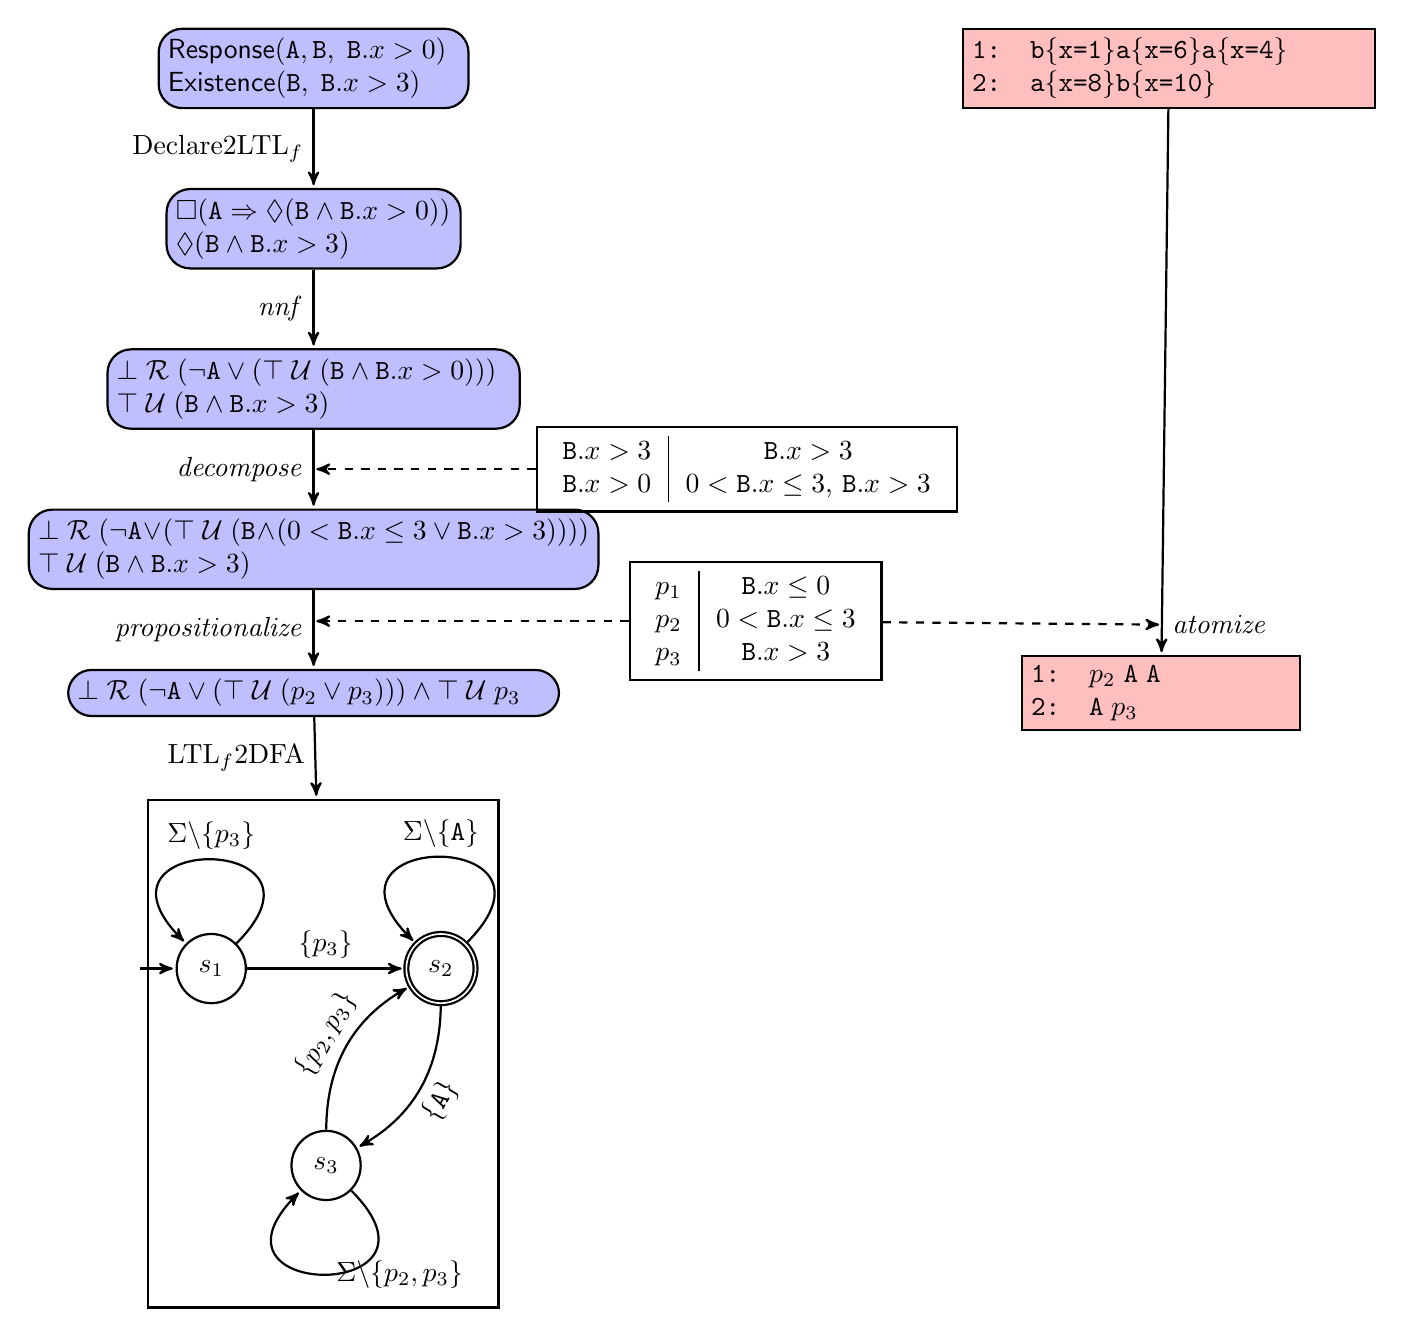
\begin{tikzpicture}[->,>=stealth',shorten >=1pt,thick,initial text=$ $]
	\node (Clause) [fill=blue!25,text width=3.7cm,rounded corners=.3cm,draw=black] {$\mathsf{Response}(\texttt{A},\texttt{B},\;\texttt{B}.x>0)$\\$\mathsf{Existence}(\texttt{B},\; \texttt{B}.x>3)$};
	\node (Traces) [fill=red!25,text width=5cm,draw=black,right=6.25cm of Clause] {\texttt{1:\quad b\{x=1\}a\{x=6\}a\{x=4\}}\\\texttt{2:\quad a\{x=8\}b\{x=10\}}};
	\node (LTLf1) [below=of Clause,fill=blue!25,text width=3.5cm,rounded corners=.3cm,draw=black] {$\square(\texttt{A}\Rightarrow \lozenge(\texttt{B}\wedge \texttt{B}.x>0))$\\$\lozenge(\texttt{B}\wedge \texttt{B}.x>3)$};
	\draw[->] (Clause) -- (LTLf1) node[midway,left] {Declare2LTL$_f$};
	\node (LTLf2) [below=of LTLf1,fill=blue!25,text width=5cm,rounded corners=.3cm,draw=black] {$\bot\; \mathcal{R}\; (\neg\texttt{A} \vee (\top\;\mathcal{U}\;(\texttt{B}\wedge \texttt{B}.x>0)))$\\$\top\;\mathcal{U}\;(\texttt{B}\wedge \texttt{B}.x>3)$};
	\draw[->] (LTLf1) -- (LTLf2) node[midway,left] {\textit{nnf}};
	\node (LTLf3) [below= of LTLf2,fill=blue!25,text width=7cm,rounded corners=.3cm,draw=black] {$\bot\; \mathcal{R}\; (\neg\texttt{A} \vee (\top\;\mathcal{U}\;(\texttt{B}\wedge \left(0<\texttt{B}.x\leq 3\vee \texttt{B}.x>3\right))))$\\$\top\;\mathcal{U}\;(\texttt{B}\wedge \texttt{B}.x>3)$};
	\node (tab1) [ shape=rectangle,draw] at ($(LTLf2)!0.5!(LTLf3)+(5.5,0)$) {
		\begin{tabular}{c|c}
		$\texttt{B}.x>3$      & $\texttt{B}.x>3$\\
		$\texttt{B}.x> 0$ & $0<\texttt{B}.x\leq 3$, $ \texttt{B}.x>3$\\
		\end{tabular}
	};
	
	\draw[->] (LTLf2) -- (LTLf3) node[midway,left] {\textit{decompose}};
	\node (LTLf4) [below= of LTLf3,fill=blue!25,text width=6cm,rounded corners=.3cm,draw=black] {$\bot\; \mathcal{R}\; (\neg\texttt{A} \vee (\top\;\mathcal{U}\;(p_2\vee p_3)))\wedge\top\;\mathcal{U}\;p_3$};
	\node (CTraces) [fill=red!25,text width=3.3cm,draw=black,right=5.85cm of LTLf4] {\texttt{1:\quad $p_2$\;\texttt{A\;A}}\\\texttt{2:\quad A}\;$p_3$};
	\draw[->] (Traces) -- (CTraces);
	\draw[->] (LTLf3) -- (LTLf4) node[midway,left] {\textit{propositionalize}};
	\draw[->,dashed] (tab1) -- ($(LTLf2)!0.5!(LTLf3)$);
	\node (tab2) [right=of LTLf3, shape=rectangle,draw] at ($(LTLf4)!0.5!(LTLf3)+(3,0)$) {
		\begin{tabular}{c|c}
		$p_1$ &  $\texttt{B}.x\leq 0$\\
		$p_2$ & $0<\texttt{B}.x\leq 3$\\
		$p_3$ &  $\texttt{B}.x>3$\\
		\end{tabular}
	};
	\draw[->,dashed] (tab2) -- ($(LTLf3)!0.5!(LTLf4)$);
	\node[state,initial] (SA) at ($(LTLf4)-(1.3,3.5)$) {$s_1$};
	\path (SA) edge[loop] node[midway,above] (W1) {$\Sigma\backslash\{p_3\}$} (SA);
	\node[state,accepting,right =2cm of SA] (ST) {$s_2$};
	\path (ST) edge[loop] node[midway,above] (W2) {$\Sigma\backslash\{\texttt{A}\}$} (ST);
	\draw[->] (SA) -- (ST) node[midway,above] {$ \{p_3\}$};
	\node[state] (bot) at ($(SA)!0.5!(ST)-(0,2.5)$) {$s_3$};
	\draw[->] (ST) edge [bend left] node[midway,below,sloped] {$\{\texttt{A}\}$}  (bot)  ; 
	\draw[->] (bot) 
	edge [bend left] node[midway,above,sloped] {$\{p_2,p_3\}$} (ST)  ;
	\draw[->,dashed] (tab2) -- ($(Traces)!(tab2.east)!(CTraces)$) node [right] {\textit{atomize}};
	\draw (bot) to [in=225,out=315,looseness=8] node[above,right] (W3) {$\Sigma\backslash\{p_2,p_3\}$} (bot);
	\node[draw=black,fit=(SA) (ST) (W1) (W2) (bot) (W3)] (NFA) {};
	\draw[->] (LTLf4) -- (NFA) node[midway,left] {LTL$_f$2DFA};
	\end{tikzpicture}
\end{document}